\section{Testing}
\label{sec:pl-test}
    Mosquito detection is an inherently binary classification task, there either is a mosquito or there is not. This defines how performance is evaluated, restricting analysis metrics to those within the binary domain. Even with the multi-class interpretation of the problem discussed in sections \ref{sec:pl-data} and \ref{sec:pl-clf} the results are still mapped back to the binary domain, as evaluating performance over multiple classes unnecessarily increases complexity and stifles comparison between two-class methods.
    \subsection{Standard Machine Learning Metrics}
    \label{subsec:pl-test-stan}
         \begin{wrapfigure}{r}{0.3\textwidth}
            \centering
            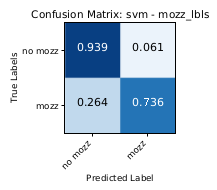
\includegraphics[width=0.3\textwidth]{conf}
            \caption{An example confusion matrix of an SVM output.}
            \label{fig:pl-test-stan-conf}
        \end{wrapfigure}
        Many performance evaluation methods exist for binary classification; the choice of `suitable' metrics depends on the context of the problem. An important attribute of the classification model is the rate at which a mosquito is correctly identified as a mosquito and the rate at which no mosquito is correctly identified as no mosquito. A \textit{confusion matrix} illustrates this, shown in figure \ref{fig:pl-test-stan-conf}. The counts for true negatives (TN), false positives (TP), false negatives (FN), and true positives (TP) are represented in matrix form in the respective order given. Normalisation can be applied row-wise or column wise giving different representations of classifier performance, this has been the source of much confusion in machine learning literature \cite{Gambino2006}. In this report, row-wise normalisation is determined to be more useful in gauging predictive accuracy and the terms are chosen to be defined as
        \begin{tgather}
            \footnotesize\text{Specificity/True Negative Rate (TNR)} = \frac{\text{TN}}{\text{TN+FP}}, \text{ Test False Positive Rate (FPR)} = \frac{\text{FP}}{\text{TN+FP}}\\
            \footnotesize\text{Miss Rate/False Negative Rate (FNR)} = \frac{\text{FN}}{\text{TP+FN}}, \text{ Sensitivity/Recall/True Positive Rate (TPR)} = \frac{\text{TP}}{\text{TP+FN}}.
        \end{tgather}
        
        \vspace{-1cm}
        Plotting the sensitivity against the false positive rate, whilst the decision boundary is varied, is informative of a classifiers performance \cite{Fawcett2005}. In this space, the \textit{Receiver Operating Characteristic} (ROC) space, a curve following the left and top borders is indicative of a good classifier and a straight line from $(0,0)$ to $(1,1)$ is equivalent to a random guess, anything below this line is considered worse than random (but can be inverted to then perform better than random). ROC curves for a collection of classifiers are shown in fig \ref{fig:exp-summary-roc}. The area of the curve (AUC) is a compact representation of the ROC space and is a measure of the classifier's discrimination ability.
        
        Another useful representation of predictive performance is a \textit{Precision-Recall} (PR) curve \cite{Raghavan1989}. Recall, explained above, can be summarised by the statement `given a mosquito is present, will the classifier detect it?'; similarly the precision can be summarised as `given a mosquito has been predicted, what is the likelihood that the prediction is correct?' and is given by $\text{precision} = \frac{\text{TP}}{\text{TP+FP}}$. Plotting a curve in the PR space as the decision threshold is varied can show differences in algorithms that ROC curves can not, especially for skewed datasets \cite{Davis}. Again, this is compactly represented by the curve's area in PR space for ease of cross-classifier comparison.
        
        The \textit{$F_1$ score} is the harmonic mean of precision and recall, $F_1 = 2\cdot\frac{\text{precision}\cdot \text{recall}}{\text{precision}+\text{recall}}$ . The harmonic mean, instead of the arithmetic or geometric mean, takes into account the magnitude of the precision and recall and also how similar they are. For example, a classifier with precision $0.7$ and recall $0.8$ has a higher $F_1$ score than a classifier with precision $0.6$ and recall $0.9$, but the arithmetic mean is the same for both.
        
        % \begin{sitemize}
        %     \item{confusion mat, roc, prec-rec, f1 score [harmonic mean, makes more sense for ratios and rates], crossval}
        %     %https://www.quora.com/What-is-an-intuitive-explanation-of-F-score
        %     \item{explain what each describes and its relevancy in this context}
        %     \item{explain significance of areas as well and how they can give good condensed idea of graph}
        %     \item{test of RFE and PCA, explain how only some classifiers can do rfe, talk about log and linear spacing}
        %     \item{', but also the area under the ROC curve (AUC), more recommended for evaluating the classification in problems involving imbalanced classes [22].'}
        % \end{sitemize}
        
    \subsection{Less-Common Machine Learning Metrics}
    \label{subsec:pl-test-less}
        Performance of the selected classifiers is boosted by a number of post-processing techniques in section \ref{sec:exp-postproc}. Because of this, metrics and visualisations are needed to gauge the effects. In terms of rejection, there are three groups of metrics. The first, and most simple, is the rejection ratio which is the number of rejected predictions over the total number of predictions, an intuitive value for this context. The next series of tests are plots of the metrics detailed above against the rejection ratio, as the rejection threshold is varied symmetrically; this can be useful for getting initial ideas how a classifier will perform with rejection and are an extension of accuracy-rejection curves (ARC) first studied by \textcite{SajjadAhmedNadeem}. The last group of rejection-based metrics visualise the asymmetrical rejection-space. On the $x$-axis, the positive class (mosquito) rejection threshold is varied and on the $y$-axis the negative class (no mosquito) threshold is varied. Below each threshold, the percentage of the respective class rejected is shown, so for any value in the grid the total rejection is the sum of the rejection for each class. These binary asymmetrical rejection grids prove useful in section \ref{subsec:exp-postproc-rej} for tuning classifier performance in reference to a given specification. Tests are also performed for filtering operations where metrics are calculated and plotted against varying kernel sizes. Examples of a rejection grid and filtering plot are shown in figures \ref{fig:exp-postproc-asymrej} and \ref{fig:exp-postproc-rejfilt} respectively.
        % \begin{sitemize}
        %     \item{rejection ratio, acc-rej plot, f1-rej plot, binary asymmetrical rejection matrix,median-f1,etc}
        %     \item{explain what each describes and its relevancy in this context}
        % \end{sitemize}
    
    \subsection{Cross Validation}
    \label{subsec:pl-test-xval}
        Every experiment in section \ref{sec:exp-clf} is cross-validated, with details and justifications regarding experimental design given in section \ref{subsec:exp-clf-xval}. The stratified $k$-fold cross validation algorithm first splits the data into positive samples and negative samples. Each group is then randomly split into $k$ groups and combined to make up $k$ folds, where the original class proportions are preserved. Experiments then train on $k-1$ folds and test on the left out fold. Cross-validation tests are implemented in `MozzPy' in such a way that the arguments for \textit{all} experiments are collected first, then they are passed to a multi-processing function that divides jobs between the specified number of cores. Scikit-learn includes a number of cross-validation tools, but these are only utilised once for recursive feature elimination, all other implementations are done manually for richer metric output and a finer degree of control.
        
    \subsection{Software Implementation}
    \label{subsec:pl-test-software}
        After tests have been carried out on multiple classifiers, the \code{ClassiSet} objects are accumulated into a \code{ResultSet} object where plotting and general information export is managed. In terms of plotting results, the parent set, \code{HumSet}, implements a \code{plot()} method. This instantiates a collection of blank figures, the number of which is determined by input arguments, which are then passed to the inheriting objects \code{subplot()} method. The \code{subplot()} method fills the figures with relevant information, possibly calling \code{subplot()} on set objects it contains, and returns the filled figures to be saved. For example, calling \code{plot()} on a \code{ResultSet} instance will call \code{subplot()} on each \code{ClassiSet} instance which fills figures with results and in calls \code{subplot()} on the contained \code{DataSet} object and goes right down to the \code{WavSet} objects.
        
        Each set of predictions are plotted below the original signal and ground truth labels, where rejection is visualised by overlaying a plot of Gaussian smoothed delta functions wherever a sample is rejected, visible in figure \ref{fig:exp-clf-summary-rej}.